

\tikzset{every picture/.style={line width=0.75pt}} %set default line width to 0.75pt        

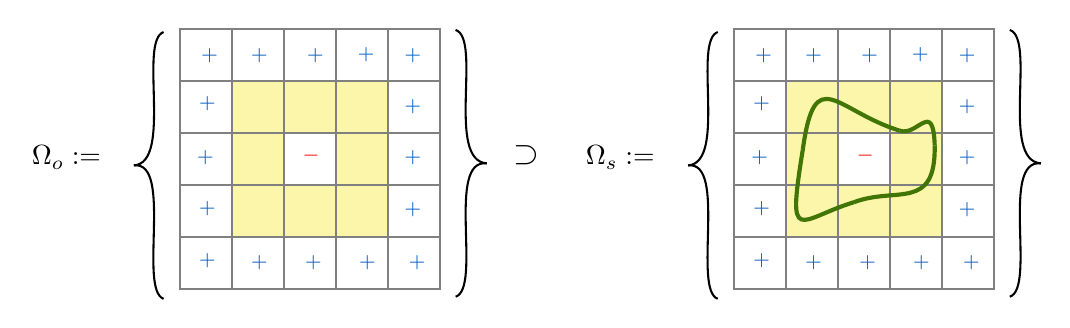
\begin{tikzpicture}[x=0.75pt,y=0.75pt,yscale=-1,xscale=1]
%uncomment if require: \path (0,192); %set diagram left start at 0, and has height of 192

%Shape: Rectangle [id:dp1875272590329995] 
\draw  [draw opacity=0][fill={rgb, 255:red, 248; green, 231; blue, 28 }  ,fill opacity=0.37 ] (288.98,76.59) -- (314.07,76.59) -- (314.07,101.69) -- (288.98,101.69) -- cycle ;
%Shape: Rectangle [id:dp45926838944511017] 
\draw  [draw opacity=0][fill={rgb, 255:red, 248; green, 231; blue, 28 }  ,fill opacity=0.37 ] (238.78,76.59) -- (263.88,76.59) -- (263.88,101.69) -- (238.78,101.69) -- cycle ;
%Shape: Rectangle [id:dp951208679037494] 
\draw  [draw opacity=0][fill={rgb, 255:red, 248; green, 231; blue, 28 }  ,fill opacity=0.37 ] (238.78,101.69) -- (314.68,101.69) -- (314.68,126.79) -- (238.78,126.79) -- cycle ;
%Shape: Rectangle [id:dp007344814580564685] 
\draw  [draw opacity=0][fill={rgb, 255:red, 248; green, 231; blue, 28 }  ,fill opacity=0.37 ] (238.78,51.5) -- (314.07,51.5) -- (314.07,76.59) -- (238.78,76.59) -- cycle ;
%Shape: Grid [id:dp3223419934026063] 
\draw  [draw opacity=0] (213.68,26.4) -- (339.17,26.4) -- (339.17,151.89) -- (213.68,151.89) -- cycle ; \draw  [color={rgb, 255:red, 128; green, 128; blue, 128 }  ,draw opacity=1 ] (238.78,26.4) -- (238.78,151.89)(263.88,26.4) -- (263.88,151.89)(288.98,26.4) -- (288.98,151.89)(314.07,26.4) -- (314.07,151.89) ; \draw  [color={rgb, 255:red, 128; green, 128; blue, 128 }  ,draw opacity=1 ] (213.68,51.5) -- (339.17,51.5)(213.68,76.59) -- (339.17,76.59)(213.68,101.69) -- (339.17,101.69)(213.68,126.79) -- (339.17,126.79) ; \draw  [color={rgb, 255:red, 128; green, 128; blue, 128 }  ,draw opacity=1 ] (213.68,26.4) -- (339.17,26.4) -- (339.17,151.89) -- (213.68,151.89) -- cycle ;
%Curve Lines [id:da008301583048880179] 
\draw    (206,28) .. controls (193.78,32.18) and (210.55,90.95) .. (191.68,92.27) ;
%Curve Lines [id:da5597728155003041] 
\draw    (206,156.53) .. controls (193.78,152.35) and (210.55,89.95) .. (191.68,92.27) ;

%Curve Lines [id:da02896941551177379] 
\draw    (346.68,27) .. controls (359.49,31.18) and (341.92,89.95) .. (361.68,91.27) ;
%Curve Lines [id:da9303782701504543] 
\draw    (346.68,155.53) .. controls (359.49,151.35) and (341.92,88.95) .. (361.68,91.27) ;

%Shape: Rectangle [id:dp8595008353400008] 
\draw  [draw opacity=0][fill={rgb, 255:red, 248; green, 231; blue, 28 }  ,fill opacity=0.37 ] (555.98,76.59) -- (581.07,76.59) -- (581.07,101.69) -- (555.98,101.69) -- cycle ;
%Shape: Rectangle [id:dp10897143783297769] 
\draw  [draw opacity=0][fill={rgb, 255:red, 248; green, 231; blue, 28 }  ,fill opacity=0.37 ] (505.78,76.59) -- (530.88,76.59) -- (530.88,101.69) -- (505.78,101.69) -- cycle ;
%Shape: Rectangle [id:dp8256281985192404] 
\draw  [draw opacity=0][fill={rgb, 255:red, 248; green, 231; blue, 28 }  ,fill opacity=0.37 ] (505.78,101.69) -- (581.68,101.69) -- (581.68,126.79) -- (505.78,126.79) -- cycle ;
%Shape: Rectangle [id:dp9508677694883004] 
\draw  [draw opacity=0][fill={rgb, 255:red, 248; green, 231; blue, 28 }  ,fill opacity=0.37 ] (505.78,51.5) -- (581.07,51.5) -- (581.07,76.59) -- (505.78,76.59) -- cycle ;
%Shape: Grid [id:dp6918715763510325] 
\draw  [draw opacity=0] (480.68,26.4) -- (606.17,26.4) -- (606.17,151.89) -- (480.68,151.89) -- cycle ; \draw  [color={rgb, 255:red, 128; green, 128; blue, 128 }  ,draw opacity=1 ] (505.78,26.4) -- (505.78,151.89)(530.88,26.4) -- (530.88,151.89)(555.98,26.4) -- (555.98,151.89)(581.07,26.4) -- (581.07,151.89) ; \draw  [color={rgb, 255:red, 128; green, 128; blue, 128 }  ,draw opacity=1 ] (480.68,51.5) -- (606.17,51.5)(480.68,76.59) -- (606.17,76.59)(480.68,101.69) -- (606.17,101.69)(480.68,126.79) -- (606.17,126.79) ; \draw  [color={rgb, 255:red, 128; green, 128; blue, 128 }  ,draw opacity=1 ] (480.68,26.4) -- (606.17,26.4) -- (606.17,151.89) -- (480.68,151.89) -- cycle ;
%Curve Lines [id:da6295844255433479] 
\draw    (473,28) .. controls (460.78,32.18) and (477.55,90.95) .. (458.68,92.27) ;
%Curve Lines [id:da968864494956809] 
\draw    (473,156.53) .. controls (460.78,152.35) and (477.55,89.95) .. (458.68,92.27) ;

%Curve Lines [id:da8514128320377528] 
\draw    (613.68,27) .. controls (626.49,31.18) and (608.92,89.95) .. (628.68,91.27) ;
%Curve Lines [id:da03483001801406849] 
\draw    (613.68,155.53) .. controls (626.49,151.35) and (608.92,88.95) .. (628.68,91.27) ;

%Curve Lines [id:da6944076159894066] 
\draw [color={rgb, 255:red, 65; green, 117; blue, 5 }  ,draw opacity=1 ][line width=1.5]    (513.94,84.76) .. controls (519.79,42.26) and (529.63,65.86) .. (560.53,75.49) ;
%Curve Lines [id:da04901172257911568] 
\draw [color={rgb, 255:red, 65; green, 117; blue, 5 }  ,draw opacity=1 ][line width=1.5]    (513.94,84.76) .. controls (506.21,132.25) and (511.69,118.26) .. (538.64,109.97) ;
%Curve Lines [id:da12532524491720676] 
\draw [color={rgb, 255:red, 65; green, 117; blue, 5 }  ,draw opacity=1 ][line width=1.5]    (538.64,109.97) .. controls (559.21,102.26) and (578.04,114.54) .. (577.5,82.61) ;
%Curve Lines [id:da17629004511076274] 
\draw [color={rgb, 255:red, 65; green, 117; blue, 5 }  ,draw opacity=1 ][line width=1.5]    (560.53,75.49) .. controls (569.08,78.76) and (576.78,59.92) .. (577.5,82.61) ;


% Text Node
\draw (320.54,34.36) node [anchor=north west][inner sep=0.75pt]  [font=\scriptsize,color={rgb, 255:red, 9; green, 96; blue, 196 }  ,opacity=1 ]  {$+$};
% Text Node
\draw (320.54,59.09) node [anchor=north west][inner sep=0.75pt]  [font=\scriptsize,color={rgb, 255:red, 9; green, 96; blue, 196 }  ,opacity=1 ]  {$+$};
% Text Node
\draw (320.54,83.38) node [anchor=north west][inner sep=0.75pt]  [font=\scriptsize,color={rgb, 255:red, 9; green, 96; blue, 196 }  ,opacity=1 ]  {$+$};
% Text Node
\draw (320.54,108.55) node [anchor=north west][inner sep=0.75pt]  [font=\scriptsize,color={rgb, 255:red, 9; green, 96; blue, 196 }  ,opacity=1 ]  {$+$};
% Text Node
\draw (322.54,134.28) node [anchor=north west][inner sep=0.75pt]  [font=\scriptsize,color={rgb, 255:red, 9; green, 96; blue, 196 }  ,opacity=1 ]  {$+$};
% Text Node
\draw (271.33,82.65) node [anchor=north west][inner sep=0.75pt]  [font=\scriptsize,color={rgb, 255:red, 255; green, 0; blue, 0 }  ,opacity=1 ]  {$-$};
% Text Node
\draw (297.98,33.8) node [anchor=north west][inner sep=0.75pt]  [font=\scriptsize,color={rgb, 255:red, 9; green, 96; blue, 196 }  ,opacity=1 ]  {$+$};
% Text Node
\draw (273.54,34.36) node [anchor=north west][inner sep=0.75pt]  [font=\scriptsize,color={rgb, 255:red, 9; green, 96; blue, 196 }  ,opacity=1 ]  {$+$};
% Text Node
\draw (246.54,34.36) node [anchor=north west][inner sep=0.75pt]  [font=\scriptsize,color={rgb, 255:red, 9; green, 96; blue, 196 }  ,opacity=1 ]  {$+$};
% Text Node
\draw (222.54,34.36) node [anchor=north west][inner sep=0.75pt]  [font=\scriptsize,color={rgb, 255:red, 9; green, 96; blue, 196 }  ,opacity=1 ]  {$+$};
% Text Node
\draw (221.54,57.36) node [anchor=north west][inner sep=0.75pt]  [font=\scriptsize,color={rgb, 255:red, 9; green, 96; blue, 196 }  ,opacity=1 ]  {$+$};
% Text Node
\draw (220.54,83.36) node [anchor=north west][inner sep=0.75pt]  [font=\scriptsize,color={rgb, 255:red, 9; green, 96; blue, 196 }  ,opacity=1 ]  {$+$};
% Text Node
\draw (221.54,108.36) node [anchor=north west][inner sep=0.75pt]  [font=\scriptsize,color={rgb, 255:red, 9; green, 96; blue, 196 }  ,opacity=1 ]  {$+$};
% Text Node
\draw (221.54,133.36) node [anchor=north west][inner sep=0.75pt]  [font=\scriptsize,color={rgb, 255:red, 9; green, 96; blue, 196 }  ,opacity=1 ]  {$+$};
% Text Node
\draw (246.54,134.36) node [anchor=north west][inner sep=0.75pt]  [font=\scriptsize,color={rgb, 255:red, 9; green, 96; blue, 196 }  ,opacity=1 ]  {$+$};
% Text Node
\draw (272.54,134.36) node [anchor=north west][inner sep=0.75pt]  [font=\scriptsize,color={rgb, 255:red, 9; green, 96; blue, 196 }  ,opacity=1 ]  {$+$};
% Text Node
\draw (298.54,134.36) node [anchor=north west][inner sep=0.75pt]  [font=\scriptsize,color={rgb, 255:red, 9; green, 96; blue, 196 }  ,opacity=1 ]  {$+$};
% Text Node
\draw (141,81.4) node [anchor=north west][inner sep=0.75pt]    {$\Omega _{o} :=$};
% Text Node
\draw (587.54,34.36) node [anchor=north west][inner sep=0.75pt]  [font=\scriptsize,color={rgb, 255:red, 9; green, 96; blue, 196 }  ,opacity=1 ]  {$+$};
% Text Node
\draw (587.54,59.09) node [anchor=north west][inner sep=0.75pt]  [font=\scriptsize,color={rgb, 255:red, 9; green, 96; blue, 196 }  ,opacity=1 ]  {$+$};
% Text Node
\draw (587.54,83.38) node [anchor=north west][inner sep=0.75pt]  [font=\scriptsize,color={rgb, 255:red, 9; green, 96; blue, 196 }  ,opacity=1 ]  {$+$};
% Text Node
\draw (587.54,108.55) node [anchor=north west][inner sep=0.75pt]  [font=\scriptsize,color={rgb, 255:red, 9; green, 96; blue, 196 }  ,opacity=1 ]  {$+$};
% Text Node
\draw (589.54,134.28) node [anchor=north west][inner sep=0.75pt]  [font=\scriptsize,color={rgb, 255:red, 9; green, 96; blue, 196 }  ,opacity=1 ]  {$+$};
% Text Node
\draw (538.33,82.65) node [anchor=north west][inner sep=0.75pt]  [font=\scriptsize,color={rgb, 255:red, 255; green, 0; blue, 0 }  ,opacity=1 ]  {$-$};
% Text Node
\draw (564.98,33.8) node [anchor=north west][inner sep=0.75pt]  [font=\scriptsize,color={rgb, 255:red, 9; green, 96; blue, 196 }  ,opacity=1 ]  {$+$};
% Text Node
\draw (540.54,34.36) node [anchor=north west][inner sep=0.75pt]  [font=\scriptsize,color={rgb, 255:red, 9; green, 96; blue, 196 }  ,opacity=1 ]  {$+$};
% Text Node
\draw (513.54,34.36) node [anchor=north west][inner sep=0.75pt]  [font=\scriptsize,color={rgb, 255:red, 9; green, 96; blue, 196 }  ,opacity=1 ]  {$+$};
% Text Node
\draw (489.54,34.36) node [anchor=north west][inner sep=0.75pt]  [font=\scriptsize,color={rgb, 255:red, 9; green, 96; blue, 196 }  ,opacity=1 ]  {$+$};
% Text Node
\draw (488.54,57.36) node [anchor=north west][inner sep=0.75pt]  [font=\scriptsize,color={rgb, 255:red, 9; green, 96; blue, 196 }  ,opacity=1 ]  {$+$};
% Text Node
\draw (487.54,83.36) node [anchor=north west][inner sep=0.75pt]  [font=\scriptsize,color={rgb, 255:red, 9; green, 96; blue, 196 }  ,opacity=1 ]  {$+$};
% Text Node
\draw (488.54,108.36) node [anchor=north west][inner sep=0.75pt]  [font=\scriptsize,color={rgb, 255:red, 9; green, 96; blue, 196 }  ,opacity=1 ]  {$+$};
% Text Node
\draw (488.54,133.36) node [anchor=north west][inner sep=0.75pt]  [font=\scriptsize,color={rgb, 255:red, 9; green, 96; blue, 196 }  ,opacity=1 ]  {$+$};
% Text Node
\draw (513.54,134.36) node [anchor=north west][inner sep=0.75pt]  [font=\scriptsize,color={rgb, 255:red, 9; green, 96; blue, 196 }  ,opacity=1 ]  {$+$};
% Text Node
\draw (539.54,134.36) node [anchor=north west][inner sep=0.75pt]  [font=\scriptsize,color={rgb, 255:red, 9; green, 96; blue, 196 }  ,opacity=1 ]  {$+$};
% Text Node
\draw (565.54,134.36) node [anchor=north west][inner sep=0.75pt]  [font=\scriptsize,color={rgb, 255:red, 9; green, 96; blue, 196 }  ,opacity=1 ]  {$+$};
% Text Node
\draw (408,81.4) node [anchor=north west][inner sep=0.75pt]    {$\Omega _{s} :=$};
% Text Node
\draw (373,81.4) node [anchor=north west][inner sep=0.75pt]  [font=\large]  {$\supset $};


\end{tikzpicture}
